%------------------------------------------------------------------------------
% Setup
%------------------------------------------------------------------------------
\documentclass[ 
	12pt,
	a4paper,
	bibliography=totoc,
	cleardoublepage=e, 
	index=totoc,
	ngerman, 
	openright
	final, 
	listof=nochaptergap,
	]{scrbook}
	
% Schriftarten
\usepackage{fontspec}

% Farben
\usepackage{color}
\usepackage[usenames,dvipsnames,svgnames,table]{xcolor}

% Sprache, Umlaute
\usepackage[english, ngerman]{babel}

% Graphiken
\usepackage{graphicx}
\usepackage{wrapfig}
\usepackage{enumitem}

% URL und Dateipfade
\usepackage[hyphens]{url}

% Deutsche Anfuehrungszeichen
\usepackage[babel, german=quotes]{csquotes}

% Seitenformatierung
\usepackage[
	portrait,
	bindingoffset=1.5cm,
	inner=2.5cm,
	outer=2.5cm,
	top=3cm,
	bottom=2cm,
	%includeheadfoot
	]{geometry}
	
% Kopf- und Fußzeilen
\usepackage{fancyhdr}

% Standard Zeilenabstand
\usepackage{setspace}

% Inhaltsverzeichnis
\usepackage{tocloft}

% Untertitel
\usepackage{caption}

% Unterdrueckung von vertikalen Linien
\usepackage{booktabs}

% Fluss eigenschaften von Tabellen
\usepackage{float}

% Longtable
\usepackage{longtable}	

% Quellcode Listings
\usepackage{listings}

% Literaturverzeichnis
\usepackage{babelbib}

% Abkürzungsverzeichnis
\usepackage[printonlyused]{acronym}

% Dokumentinterne Links
\usepackage{array}

% for testing
\usepackage{lipsum}

% overfull hbox fix
\usepackage{hyphenat}

% links im toc
\usepackage{hyperref}
\hypersetup{
    colorlinks,
    citecolor=black,
    filecolor=black,
    linkcolor=black,
    urlcolor=black
}

% Untwrschriften
\newcommand*{\signaturefield}[1]{%
	\vspace{1.5cm}%
    \par\noindent\makebox[2.5in]{\hrulefill} \hfill\makebox[2.0in]{\hrulefill}%
    \par\noindent\makebox[2.5in][l]{#1}      \hfill\makebox[2.0in][l]{Datum}%
}

% Kopf- und Fußzeilen
\pagestyle{fancy}
\fancyhf{}
\fancyhead[EL,OR]{\sffamily\thepage}
\fancyhead[ER,OL]{\sffamily\leftmark}

\fancypagestyle{headings}{}

\fancypagestyle{plain}{}

\fancypagestyle{empty}{
  \fancyhf{}
  \renewcommand{\headrulewidth}{0pt}
}

% Kein "Kapitel # NAME" in der Kopfzeile
\renewcommand{\chaptermark}[1]{
	\markboth{#1}{}
   	\markboth{\thechapter.\ #1}{}
}

% Zeilenabstand: 1,5
\onehalfspacing 

% Akzentfarbe
\definecolor{akzent}{RGB}{133,60,46}

% Schriften
\newfontfamily\corpoSfamily{Helvetica}
\newfontfamily\corpoAfamily{Helvetica}
\setmainfont{Helvetica}

\addtokomafont{chapter}{\corpoAfamily\LARGE} 
\addtokomafont{section}{\corpoSfamily\Large\color{akzent}} 
\addtokomafont{subsection}{\corpoSfamily\large\mdseries} 
\addtokomafont{subsubsection}{\corpoSfamily\normalsize\mdseries}
\addtokomafont{caption}{\corpoSfamily\normalsize\mdseries} 

% Schriften im IHV
\renewcommand{\cftchapfont}{\sffamily\normalsize}
\renewcommand{\cftsecfont}{\sffamily\normalsize}
\renewcommand{\cftsubsecfont}{\sffamily\normalsize}
\renewcommand{\cftchappagefont}{\sffamily\normalsize}
\renewcommand{\cftsecpagefont}{\sffamily\normalsize}
\renewcommand{\cftsubsecpagefont}{\sffamily\normalsize}

% Zeilenabstand in den Verzeichnissen einstellen
\setlength{\cftparskip}{.5\baselineskip}
\setlength{\cftbeforechapskip}{.1\baselineskip}

% Einrücken von Absätzen deaktivieren
\setlength{\parindent}{0pt}

% Listings
\definecolor{codegreen}{rgb}{0,0.6,0}
\definecolor{codegray}{rgb}{0.5,0.5,0.5}
\definecolor{codepurple}{rgb}{0.58,0,0.82}
\definecolor{backcolour}{rgb}{0.95,0.95,0.92}
 
\lstdefinestyle{codestyle}{
	backgroundcolor=\color{backcolour},   
    commentstyle=\color{codegreen},
    keywordstyle=\color{magenta},
    numberstyle=\tiny\color{codegray},
    stringstyle=\color{codepurple},
    basicstyle=\footnotesize,
    breakatwhitespace=false,         
    breaklines=true,                 
    captionpos=b,                    
    keepspaces=true,                 
    numbers=left,                     
    numbersep=5pt,                  
    showspaces=false,                
    showstringspaces=false,
    showtabs=false,                  
    tabsize=2
}

\lstset{style=codestyle}

\lstdefinelanguage{JavaScript}{
	keywords={break, case, catch, continue, debugger, default, delete, do, else,
	finally, for, function, if, in, instanceof, new, return, switch, this, throw,
	try, typeof, var, void, while, with}, morecomment=[l]{//},
	morecomment=[s]{/*}{*/}, morestring=[b]',
	morestring=[b]",
	sensitive=true
}

% include für Visio Dokumente. 1cm Rand wird weggeschniten
\newcommand{\includevisio}[2][]{\includegraphics[clip, trim=1cm 1cm 1cm 1cm, #1]{#2}} 


%------------------------------------------------------------------------------
% Dokument
%------------------------------------------------------------------------------
\begin{document}

\setcounter{secnumdepth}{3}
 
% Titelblatt
\begin{titlepage}
\pagestyle{empty}

% ##################################################
% HFU-Logo einbinden
% ##################################################
\begin{center}

\includegraphics[height=2cm]{content/graphics/sjtubannerred.pdf}
\end{center}

\vspace{20 mm}

% ##################################################
% Titel
% ##################################################
\begin{center}
{\fontspec{CorpoA}\fontsize{28}{28} \selectfont
\textbf{Project Documentation}}\\[5mm] 
{\fontspec{Helvetica}\fontsize{16}{22}
\selectfont Project Workshop of Database Systems (CS356)\\Project my-meal.com}
\end{center}

% ##################################################
% Zusatzinformationen
% ##################################################
\vfill
\begin{tabular}{lcl}
Authors     &&    Name 1 (Student ID 1)\\ 
            &&    email1@example.com\\
            &&    Name 2 (Student ID 1)\\
            &&    email2@example.com\\
            &&    Christian Würthner\\
            &&    c.wuerthner@me.com\\\\
Professor   &&    Dr. Fang Li\\ 
            &&    Associate Prof.\\
            &&    Shanghai Jiaotong University\\
            &&    li-fang@cs.sjtu.edu.cn\\\\
Date	        &&    \today\\ 
\end{tabular}
\end{titlepage}
\cleardoubleemptypage

\frontmatter

% Inhaltsverzeichnis
\tableofcontents
\addcontentsline{toc}{chapter}{Table of Contents}
\cleardoubleemptypage

% Abbildungsverzeichnis einbinden und ins Inhaltsverzeichnis
% WORKAROUND: tocloft und KOMA funktionieren zusammen nicht
% korrekt\phantomsection
\addcontentsline{toc}{chapter}{\listfigurename} 
\listoffigures
\cleardoubleemptypage

% Abkürzungsverzeichnis
\include{framework/abbreviations}

\mainmatter

% Inhalt
\chapter{Examples}

%=======================================================================================
\section{Example Section}

%---------------------------------------------------------------------------------------
\subsection{Example Subsection}

%---------------------------------------------------------------------------------------
\subsubsection{Example Subsubsection}

%=======================================================================================
\section{Listings}
In listing \ref{example_listing} you can see the usage of an image.
\begin{figure}
\lstset{language=php}
\begin{lstlisting}
<?php
    $hello = "Hello {$_GET['name']}";
    echo $hello;
?>
\end{lstlisting}
\caption{This is the caption for the example listing. (Extract from \texttt{hello.php})}
\label{example_listing}
\end{figure}

%=======================================================================================
\section{Graphics}
In figure \ref{example_image} you can see the usage of an image.
\begin{figure}

\includegraphics[width=\textwidth]{content/graphics/example.jpg}
\caption{This is the caption for the example image}
\label{example_image}
\end{figure}

%=======================================================================================
\section{Lists}
This is a basic list
\begin{itemize}
\item First item
\item Second item
\item Third item
\end{itemize}

\chapter{Project Description}
Our project is an implementation of a food delivery system called MyMeal accessible as
a web page. It offers important features like 
searching for restaurants and for food available for ordering, or an ordering
process for customers. We have three kinds of user in our system: visitor, customer and restaurant.
A visitor is a person visiting our web page having no session id. A customer is already a
registered user with the possibility to order food. A restaurant is also a
registered user, who represents the restaurant with its menu.

\begin{figure}[hb]
	\centering
		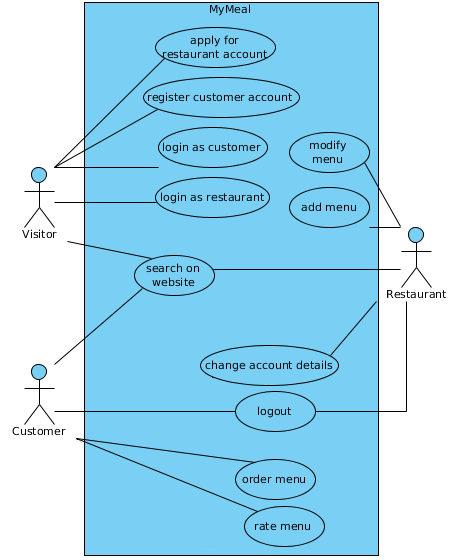
\includegraphics[scale=0.7]{content/graphics/usecase_diagram.png}
	\caption{Use case diagram of our system.}
    \label{fig:usecase_diagram}
\end{figure}


The possiblites of the users of our system are shown in figure \ref{fig:usecase_diagram}. A visitor of our website can search on it, log in as a customer or
as a restaurant, register an customer account and also apply for a restaurant account.
For now the application of a restaurant account will be processed by our similar to the
registration of a customer account. That means every restaurant will be accepted.
The application process is an optional goal.

An user logged in as a customer has the following possibilities: search
for restaurants or menus, rate a menu after it was
delivered, modify his/her rating his rating, modifying account details and
order a menu.

An user logged in as a restaurant will be able to add and modify 
his/her menus as well as the restaurant's account details 
and will also be able to search for restaurants or menus.

Optional goals: An application process for the restaurants, with 
approvement of an additional kind of user with administrative rights.
The option for a restaurant to accept or cancel an order.
The option for a customer to cancel a yet non accepted offer.
In addition we would like to offer an recommendation system for the customers based on the customer's
previous orders and ratings using machine learning techniques like neural networks
and gradient boosting.

\chapter{State of the Art}
\lipsum
\chapter{System Overview}
\lipsum
\chapter{Database}

In this chapter we introduce the different methods we considered for a database representation and give reasons for final choice we made. Then we give a detailed description for our ER model.

%=======================================================================================
\section{Selection of the Database System}
For our database we considered NoSQL and SQL methods. We looked at different NoSQL solutions like MongoDB and CouchDB.
Since nobody who was responsible for the database had experience with NoSQL wo chose to stick with the SQL approach. We  wanted to build a slim system. Therefore we first started to use SQLite. At this time we still used Python in the backend. Later in our project Python became no possibility for us anymore so moved to PHP. This also meant that we would change our SQLite system to MySQL, because one of our group members already had experience with this combination. After considering different possibilities we finally arrived back at the standard solution for a database. The advantages fast, ... %TODO 
On the clumsy, often the solutions are too complex for uncomplicated problems...%TODO


%=======================================================================================
\section{ER-Model}
	For the database of our MyFood webpage service we created the following ER model.
	%Image from ER model, for a faster compilation time it is commented out
	%\begin{figure}[h!]
	%	\centering
	%		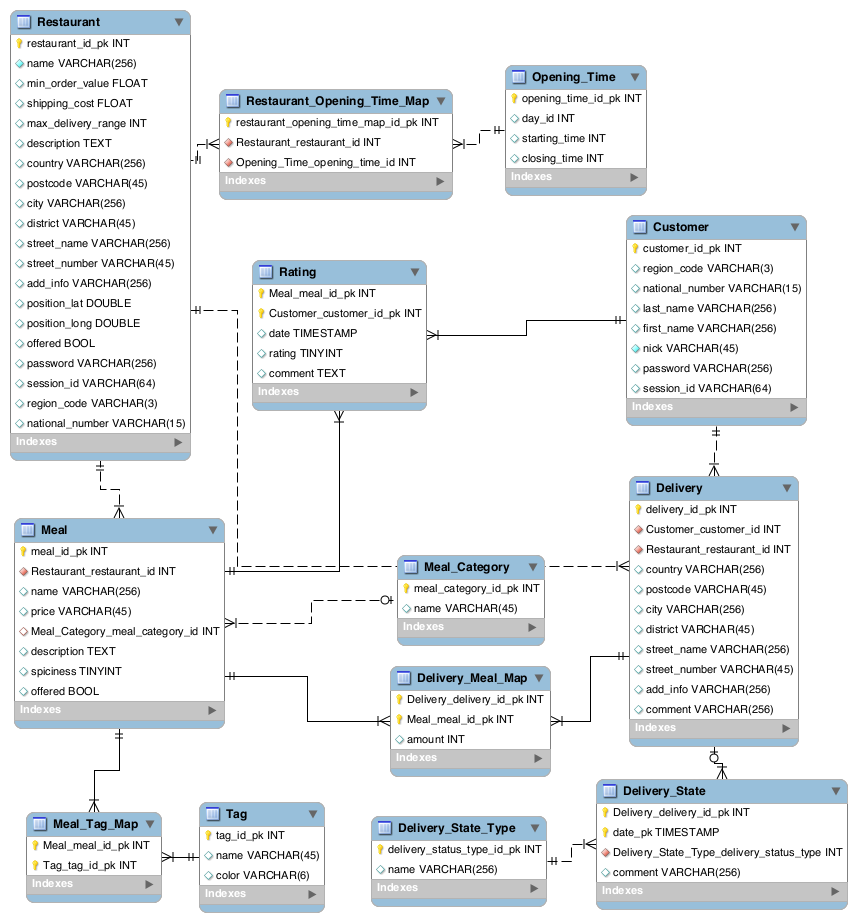
\includegraphics[scale=0.5]{content/graphics/er_model.png}
	%	\caption{ER model of our database.}
	%\end{figure}

	\subsection{Restaurant}
	The restaurant table represents the data of restaurant in real world.

	\setdescription{itemsep=5pt,parsep=0pt,leftmargin=0.5cm, style=sameline}
	\begin{description}
		\item[restaurant\_id\_pk: INT] This an automaticly generated surrogate key.
		\item[name: VARCHAR(256)] The name of the restaurant.
		\item[min\_order\_value: FLOAT] This value describes the minimum amount of value of a delivery so that a customer can submit a delivery.
	\end{description}

	\subsection{Delivery\_State}
	delivery state should be uniquely identified with the Delivery and time



%=======================================================================================
\section{Approach to our Solution}
Our first approach was to use SQLite for the database. For the communication between the database and the frontend we wanted to use the REST API framework eve\cite{python-eve}. While trying to build up a server with eve we figured out that the framework is not in a state where it is usable for our project. That is the reason we went for PHP for the interface between frontend and backend. Since it is more convenient to use PHP with MySQL we also changed the database system to MySQL.

%=======================================================================================
\section{Implementation}
We implemented for each commucation between the frontend and backend an own php file. In there we grab the content of the JSON file the frontend sends, check if the needed parameter are given and escape them. Further we prepare the needed SQL queries and inserts for the MySQL server, bind the needed paramaters and execute the SQL requests. The needed results are fetched and wrapped in an answer array and are sended back to the frontend.

%=======================================================================================
\section{Security}
\lipsum

\chapter{The RESTful Interface}
\lipsum
\chapter{Frontend}

%=======================================================================================
\section{Overview}
\lipsum

%=======================================================================================
\section{mplementation}
\lipsum

%=======================================================================================
\section{Communication with the RESTful Interface}
\lipsum

% Literaturverzeichnis
\singlespacing
\bibliographystyle{alphadin}
\bibliography{bibtex}

\appendix
\include{content/anhang}
% Hier können Anhaenge angefuegt werden

\end{document}
